\section{Results}\label{sec:results}

\subsection{Descriptive overview}
The 81 \tipi{} span 89.3 million hectares, of which 86.5 million hectares (97\%) carried tree cover above 30\% in 2000; the median territory held 403{,}600\,ha of tree cover (Table~\ref{tab:descriptive}). Forest loss inside \tipi{} over 2000--2023 totalled 1.53 million hectares, against 2.88 million hectares in the immediately surrounding 0--10\,km rings and 16.3 million hectares in the 10--50\,km rings.

\begin{table}[htbp]
\centering
\caption{Forest-cover loss 2000--2023 by zone and group. Loss share is the fraction of year-2000 tree cover (canopy $>$30\%) lost; IQR in brackets. ``Controls'' are matched non-isolated Indigenous Lands (inside zone only shown; $n=155$).}
\label{tab:descriptive}
\small
\begin{tabular*}{\columnwidth}{@{\extracolsep{\fill}} l l r r r r}
\toprule
Group & Zone & $n$ & Median loss share & Mean & Total loss (ha) \\
\midrule
TIPI & Inside & 81 & 1.01\% [0.29--3.45] & 3.13\% & 1{,}533{,}682 \\
TIPI & 0--10 km ring & 81 & 3.66\% [0.83--14.50] & 9.98\% & 2{,}880{,}999 \\
TIPI & 10--50 km ring & 81 & 5.30\% [1.22--17.87] & 10.98\% & 16{,}344{,}613 \\
Controls & Inside & 155 & 2.51\% [0.92--7.29] & 6.75\% & 1{,}006{,}569 \\
Controls & 0--10 km ring & 155 & 11.04\% [2.54--25.58] & 15.71\% & 3{,}510{,}624 \\
Controls & 10--50 km ring & 155 & 12.05\% [2.34--25.93] & 15.69\% & 25{,}010{,}799 \\
\bottomrule
\end{tabular*}


\end{table}

\subsection{RQ1: inside versus rings and matched controls (H1)}
Forest loss inside \tipi{} is far lower than immediately outside (Figure~\ref{fig:paired}). The median territory lost 1.01\% of its year-2000 tree cover internally, versus 3.66\% in its 0--10\,km ring and 5.30\% in the 10--50\,km ring. The paired differences are strongly significant and large: Wilcoxon signed-rank $W=274$, $p=6.7\times10^{-11}$ (inside vs.\ 0--10\,km; Holm-adjusted $p=2.67\times10^{-10}$; Cohen's $d_z=-0.725$; rank-biserial $r=-0.835$) and $W=149$, $p=1.11\times10^{-12}$ (inside vs.\ 10--50\,km; adjusted $p=5.53\times10^{-12}$; $d_z=-0.833$; $r=-0.910$). On average, the immediate ring lost 3.6 times more of its tree cover than the territory it surrounds; the wider ring lost 5.3 times more.

Relative to matched non-isolated Indigenous Lands, \tipi{} also fared better: median inside loss share 1.01\% versus 2.51\% for controls (Mann--Whitney $U=4252$, $p=4.77\times10^{-5}$; Holm-adjusted $p=9.54\times10^{-5}$; rank-biserial $r=-0.323$). The controls' own 0--10\,km rings lost a median 11.04\%, indicating that the region around a randomly matched Indigenous Land is under roughly three times the pressure of the region around a \tipi{} --- consistent with the remoteness of \tipi{} documented in Section~\ref{sec:access}.

A sensitivity analysis restricted to the 32 territories with explicit record-to-territory linkage (the strictest definition of hosting uncontacted peoples) strengthens every contrast: median inside loss 1.33\% versus 9.77\% (0--10\,km) and 13.6\% (10--50\,km) in rings (Wilcoxon $W=47$, $p=9.9\times10^{-6}$ and $W=9$, $p=1.5\times10^{-8}$).

\begin{figure}[t]
\centering
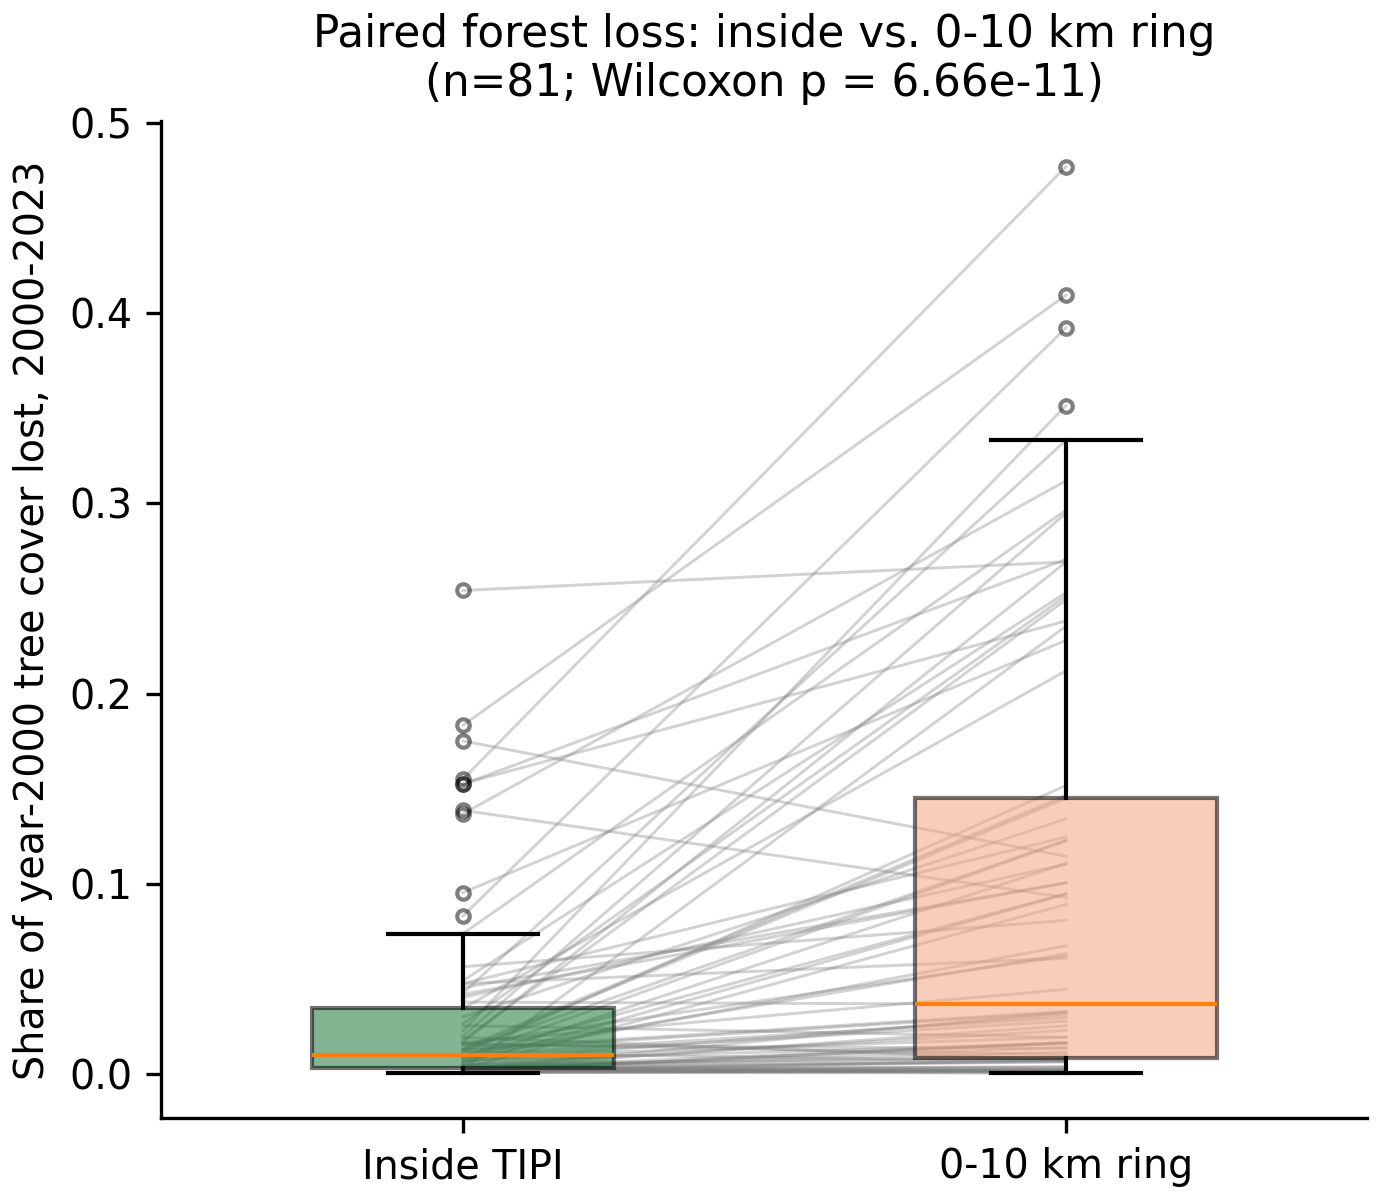
\includegraphics[width=0.62\columnwidth]{figures/fig2_paired_zones.png}
\caption{Paired forest-loss shares (fraction of year-2000 tree cover lost 2000--2023) inside \tipi{} versus their 0--10\,km rings. Grey lines connect paired values for each of the $n=81$ territories.}
\label{fig:paired}
\end{figure}

\begin{figure}[t]
\centering
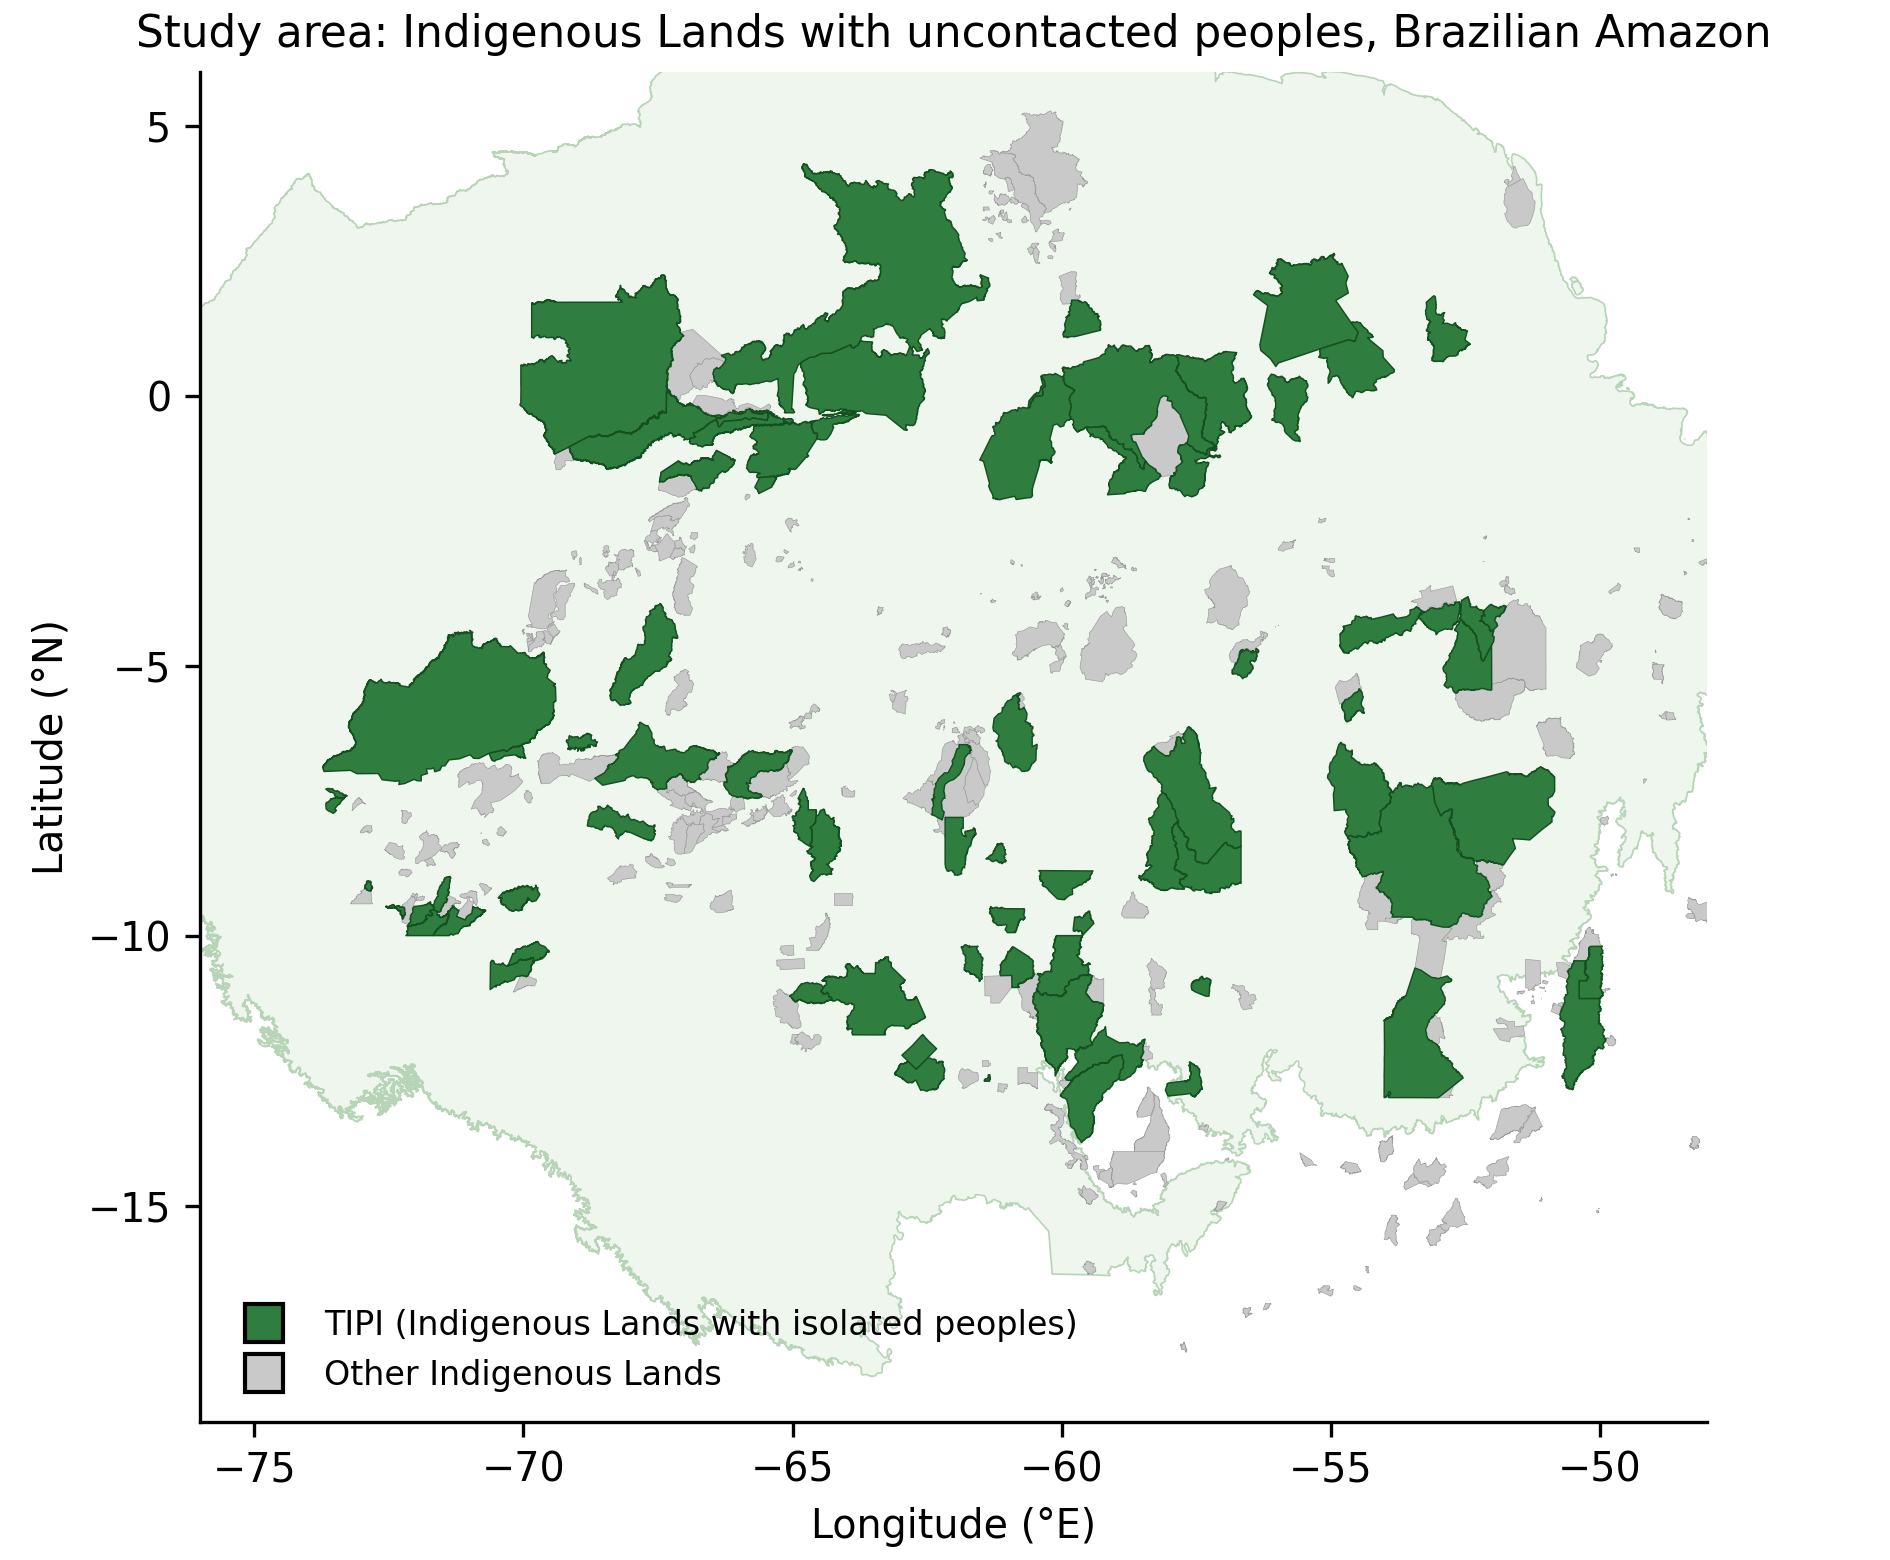
\includegraphics[width=0.8\columnwidth]{figures/fig1_study_area.png}
\caption{Study area. Green polygons are the 81 Indigenous Lands with isolated-peoples presence (\tipi{}); grey polygons are other official FUNAI Indigenous Lands within the analysis extent. Map coordinates are approximate; no settlement or record locations are shown.}
\label{fig:area}
\end{figure}

\subsection{Annual trajectories}
Inside loss was negligible and stable through 2015 (below 0.08\% of tree cover per year), then rose sharply in 2016 (0.41\%) --- a year combining a severe drought-fire season with national environmental-governance deterioration --- and remained elevated through 2023 (0.06--0.18\% per year). Aggregate inside loss more than tripled between the decades: 3.75 million loss pixels in 2001--2010, 10.5 million in 2011--2018, and 5.9 million in the five years 2019--2023. Ring trajectories mirror the same 2016--2017 peak (up to 0.73\% per year in the 10--50\,km ring), indicating that the pressure regime around these territories intensified across the board rather than only at their edges (Figure~\ref{fig:annual}).

\begin{figure}[t]
\centering
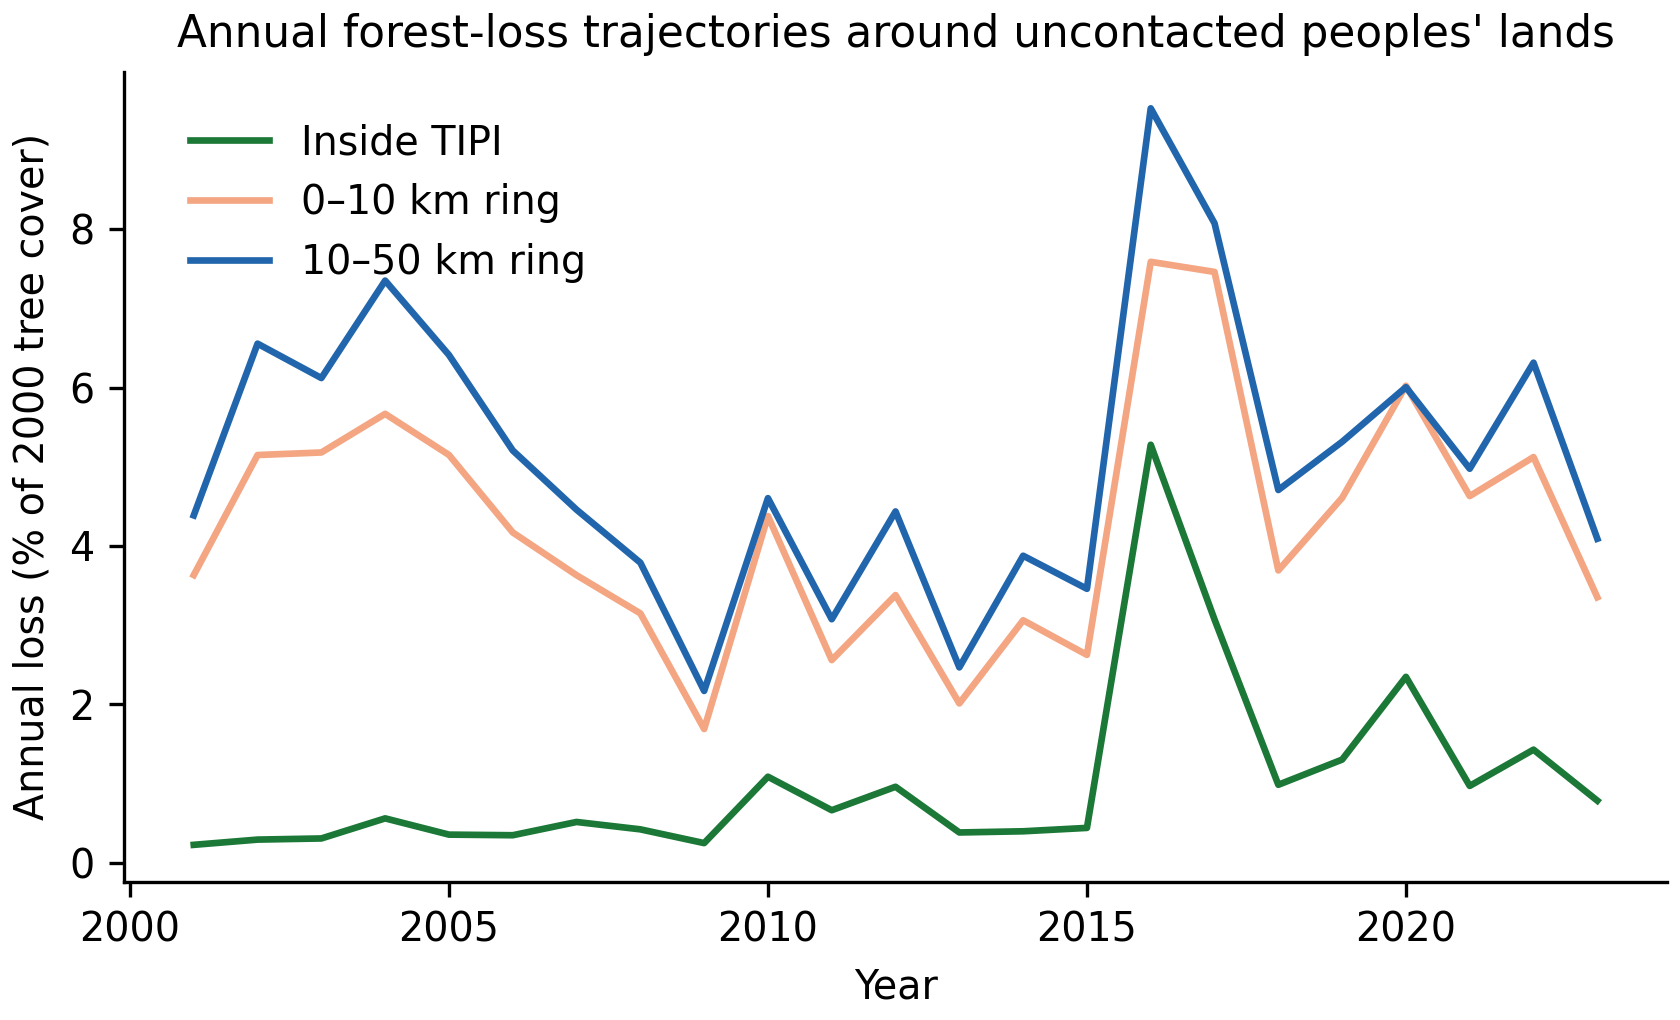
\includegraphics[width=0.85\columnwidth]{figures/fig3_annual_curves.png}
\caption{Annual forest loss as a percentage of year-2000 tree cover, aggregated across the 81 \tipi{} for each zone.}
\label{fig:annual}
\end{figure}

\subsection{RQ2: accessibility (H2)}\label{sec:access}
Ring-level pressure around \tipi{} is strongly associated with distance to the nearest city ($\rho=-0.457$, $p=1.81\times10^{-5}$; Holm-adjusted $p=5.43\times10^{-5}$; Figure~\ref{fig:access}). Conversely, distance to linear pipeline and utility corridors shows no significant correlation with ring pressure ($\rho=-0.158$, $p=0.159$; adjusted $p=0.159$). This contrast is revealing: diffuse settlement frontiers, logging access roads, and riverine trading posts centered on municipal urban hubs drive the active clearing of buffer rings, whereas isolated utility rights-of-way do not independently structure landscape deforestation.

\begin{figure}[t]
\centering
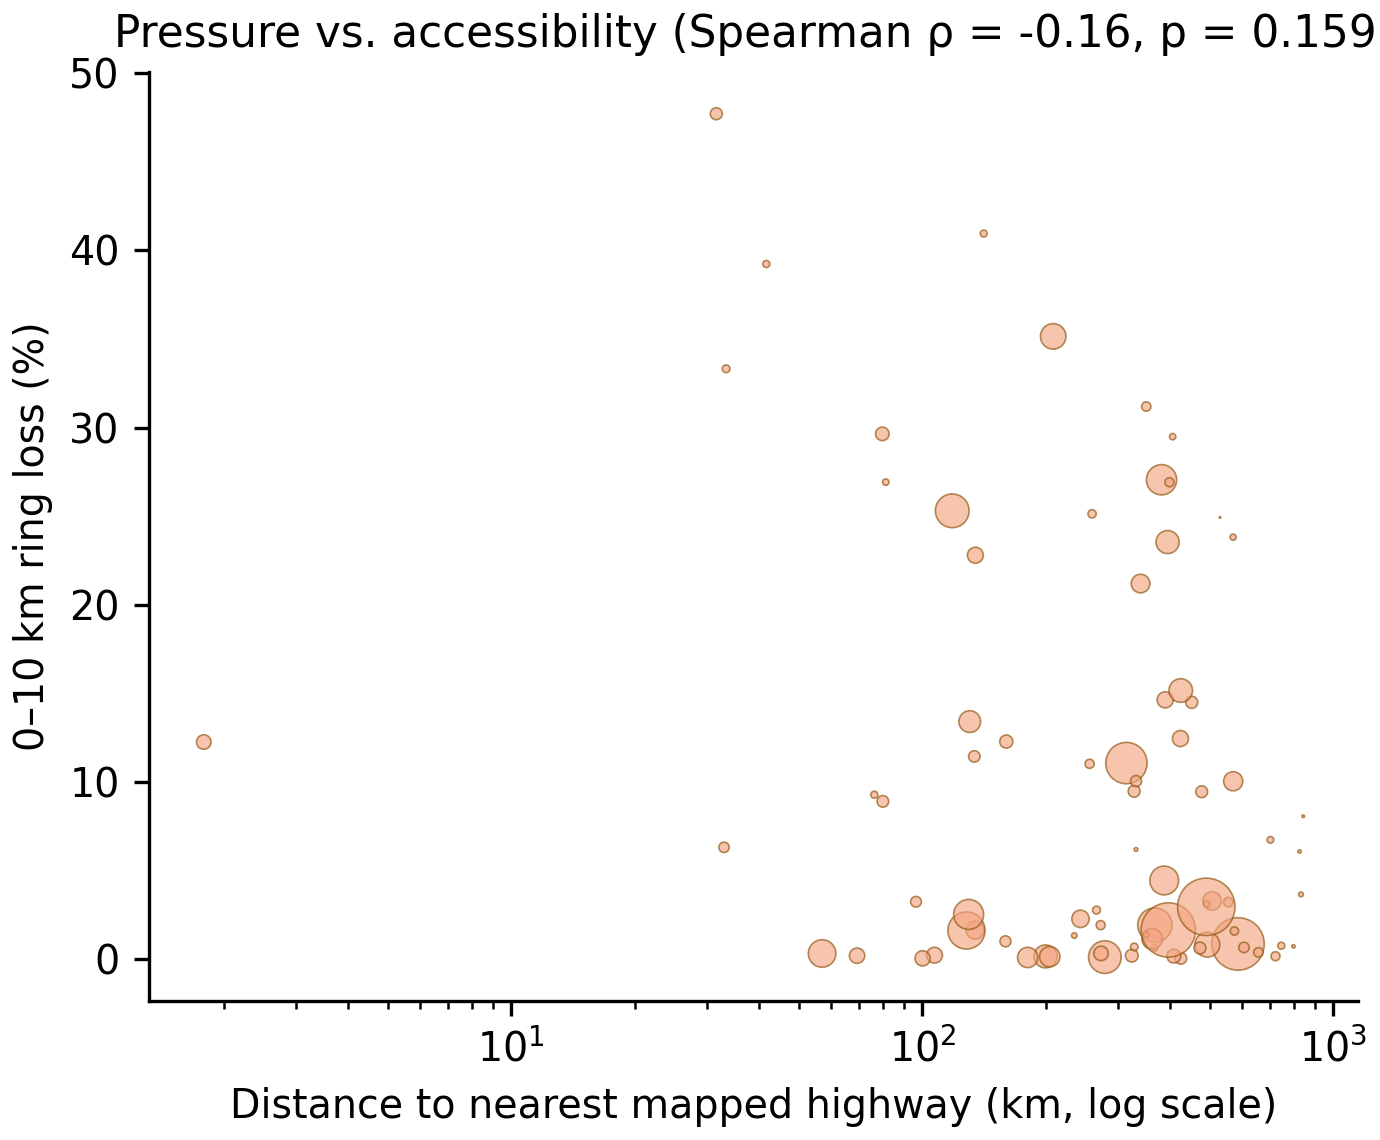
\includegraphics[width=0.62\columnwidth]{figures/fig5_accessibility.png}
\caption{0--10\,km ring loss share versus distance to the nearest mapped utility corridor (log scale); point area proportional to territory size.}
\label{fig:access}
\end{figure}

\subsection{RQ3: concentration and hotspots (H3)}
Pressure is highly concentrated. The Gini coefficient of absolute 0--10\,km ring loss across the 81 \tipi{} is 0.631 (Gini of loss share: 0.607); the top quintile of territories holds 63.5\% of aggregate ring loss, and the ten highest-pressure territories alone account for 48.5\% (Table~\ref{tab:top10}).

Examining these top-pressure territories reveals the profound buffering power of demarcation under extreme external threat (Table~\ref{tab:top10}). Uru-Eu-Wau-Wau (Rond\^onia) experienced the highest absolute external destruction, losing 222{,}349\,ha in its immediate 0--10\,km buffer ring (35.15\% of the ring's tree cover), yet deforestation inside the territory was restricted to 2.27\% (41{,}654\,ha out of 1.83 million hectares). Even more dramatically, Ba\'u (Par\'a) was besieged by 153{,}702\,ha of external clearing in its ring (23.54\% ring loss share), but suffered merely 0.25\% forest loss internally (3{,}808\,ha). In territories undergoing severe illegal invasion fronts, such as Arariboia in Maranh\~ao (15.50\% inside loss vs.\ 47.71\% in its ring) and Parque do Xingu in Mato Grosso (15.23\% inside loss vs.\ 27.06\% ring loss), internal clearing, while deeply alarming for isolated inhabitants, remained substantially lower than the near-total conversion of surrounding lands. Flagship uncontacted reserves such as Massaco (1.25\% inside loss) and Rio Omer\^e (0.59\% inside loss, surrounded by a 26.6\% ring) demonstrate that dedicated protection can halt clearing even in critical agricultural frontiers.

\begin{table}[htbp]
\centering
\caption{Ten highest-pressure \tipi{} ranked by absolute forest loss in the surrounding 0--10\,km ring, 2000--2023.}
\label{tab:top10}
\small
\begin{tabular*}{\columnwidth}{@{\extracolsep{\fill}} l l r r r r}
\toprule
Territory & State & Official Area (M ha) & 0--10\,km Ring Loss (ha) & Ring Loss Share (\%) & Inside Loss Share (\%) \\
\midrule
Uru-Eu-Wau-Wau & RO & 1.87 & 222{,}349 & 35.15 & 2.27 \\
Parque do Xingu & MT, PA & 2.64 & 201{,}849 & 27.06 & 15.23 \\
Kayap\'o & PA & 3.28 & 184{,}581 & 25.31 & 4.91 \\
Ba\'u & PA & 1.54 & 153{,}702 & 23.54 & 0.25 \\
Menkragnoti & PA, MT & 4.91 & 123{,}626 & 11.08 & 0.64 \\
Arariboia & MA & 0.41 & 112{,}000 & 47.71 & 15.50 \\
Cachoeira Seca & PA & 0.73 & 108{,}125 & 22.84 & 9.54 \\
Nambikwara & MT & 1.01 & 105{,}702 & 21.21 & 3.45 \\
Parque do Aripuan\~a & MT, RO & 1.60 & 101{,}597 & 15.17 & 1.08 \\
Yanomami & RR, AM & 9.66 & 83{,}290 & 3.01 & 1.01 \\
\bottomrule
\end{tabular*}


\end{table}

\begin{figure}[t]
\centering
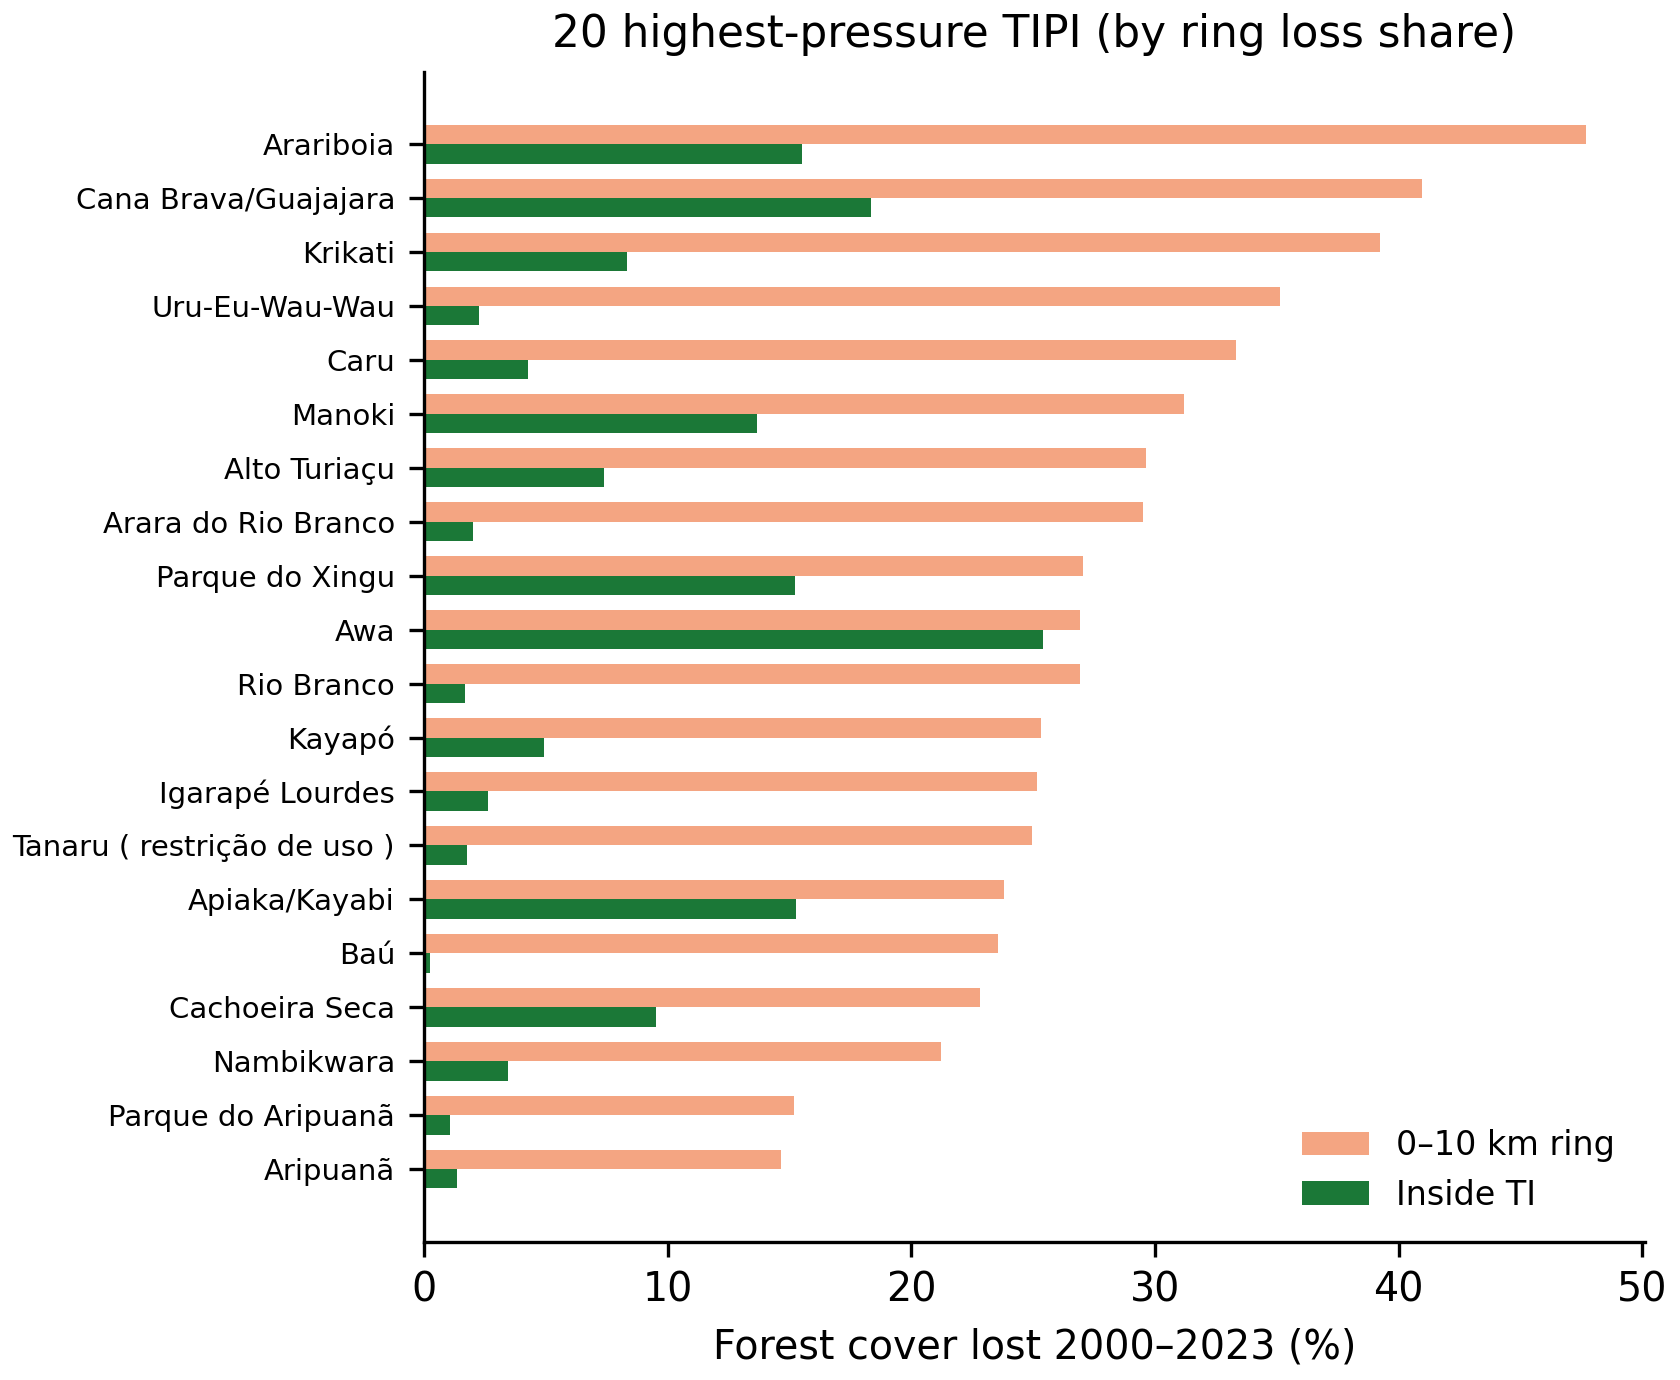
\includegraphics[width=0.8\columnwidth]{figures/fig4_top_pressure.png}
\caption{Twenty highest-pressure \tipi{} ranked by 0--10\,km ring loss share (sand), with inside loss share (green) overlaid.}
\label{fig:top}
\end{figure}

\section{Discussion}\label{sec:discussion}

\subsection{Interpretation}
Three findings stand out. First, the lands of uncontacted peoples are, quantitatively, the best-buffered Indigenous Lands in the Brazilian Amazon: 1.01\% median internal loss over 24 years, 3.6 times below their immediate surrounding rings, 5.3 times below their wider landscape buffers, and 2.5 times below matched non-isolated controls. Given that these territories host the only human populations for whom forest loss translates directly into existential risk, this asymmetry demonstrates the monumental protective success of formal demarcation and autonomous Indigenous monitoring.

Second, this buffer is under intense and concentrated pressure. External deforestation is not evenly dispersed; nearly half of all surrounding loss is concentrated around just ten territories in the soy and cattle frontiers of Rond\^onia, Par\'a, Mato Grosso, and Maranh\~ao. 

Third, the finding that municipal city distance ($\rho = -0.457$) strongly correlates with external pressure confirms that deforestation expands along diffuse agricultural and settlement frontiers. Where formal territorial protection is weakened by staffing deficits --- as documented by FUNAI's 2024 audit noting 74 vacant field posts and 12 unprotected records --- external buffer loss directly threatens the territorial integrity of uncontacted groups.

